\documentclass[letterpaper, 12pt]{article}

\usepackage{titling}
\usepackage[margin=2cm]{geometry}

\usepackage[colorlinks=true]{hyperref}

\usepackage{graphicx}

\usepackage{enumitem}

\usepackage{fontawesome5}

\usepackage{tikz}

% Title (author name and rule)

\newcommand{\name}{
    {\Large\bfseries\MakeUppercase{\theauthor}}
}

\renewcommand{\maketitle}{
    \begin{center}
        \name
    \end{center}
}

% Contact info

\newcommand{\emailnoref}{alejandrogomeznoe@gmail.com}
\newcommand{\email}{\href{mailto:\emailnoref}{\emailnoref}}

\newcommand{\linkedinpage}{\href{https://www.linkedin.com/in/alejandro-g\%C3\%B3mez-bb4239224/}{Alejandro Gómez}}
\newcommand{\githubpage}{\href{https://github.com/algono}{algono}}
\newcommand{\gitlabpage}{\href{https://gitlab.com/algono}{algono}}

% Iconos
\newcommand{\iconoDireccion}{\faIcon{map-marker-alt}}
%\newcommand{\iconoTelefono}{\faPhone}
\newcommand{\iconoTelefono}{\faIcon{phone-alt}}
\newcommand{\iconoEmail}{\faEnvelope}
\newcommand{\iconoNacionalidad}{\faGlobe}
\newcommand{\iconoFechaNacimiento}{\faBirthdayCake}
\newcommand{\iconoDni}{\faIdCard}
\newcommand{\iconoGitHub}{\faGithub}
\newcommand{\iconoGitLab}{\faGitlab}
\newcommand{\iconoLinkedin}{\faLinkedin}

\newcommand{\contactinfo}{
    \begin{minipage}[l]{.25\textwidth}
        \begin{tikzpicture}
        \clip (0,0) circle (2cm) ;
        \node[anchor=center] at (0,0) {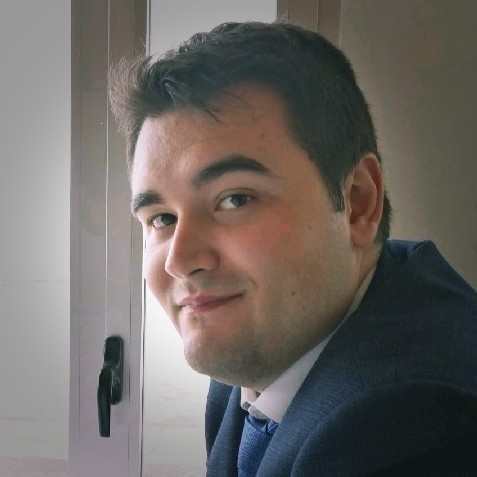
\includegraphics[width=4cm,height=4cm,keepaspectratio]{mi-foto.jpg}};
        \end{tikzpicture}
    \end{minipage}
    \begin{minipage}[r]{.6\textwidth}
        \begin{large}
            \iconoEmail \hspace{.5em} \email \par
            \vspace{12pt}
            \iconoDireccion \hspace{.5em} Mislata, Valencia \par
            \vspace{12pt}
            \iconoLinkedin \hspace{.5em} \linkedinpage \hspace{1em}
            \iconoGitHub \hspace{.5em} \githubpage \hspace{1em} \iconoGitLab \hspace{.5em} \gitlabpage
        \end{large}
    \end{minipage}
    \begin{center}
    Alejandro Gómez es un \textbf{Ingeniero Software},\\\textbf{recién licenciado} en el Grado de \textbf{Ingeniería Informática}\\ por la \textbf{\uni} (2021).
    \end{center}
}

% Other info
\newcommand{\uni}{Universitat Politècnica de València (UPV)}

\newcommand{\fce}{\emph{First Certificate in English - Cambridge}}

% My Grades

\newcommand{\gradesinyear}[2]{
    \begin{itemize}
        \item Nota media: #1
        \item Matrículas de honor: #2
    \end{itemize}
}

\newcommand{\unigrades}[9]{

    \fbox{\begin{minipage}{20em}
        \begin{center}
            \vspace{.7em}

            \textbf{Expediente}
    
            \begin{enumerate}[left=1em,
                label=\arabic*\textdegree curso:]
                \item
                    \gradesinyear{#1}{#2}
                \item
                    \gradesinyear{#3}{#4}
                \item
                    \gradesinyear{#5}{#6}
                \item
                    \gradesinyear{#7}{#8}
            \end{enumerate}

            Nota final (TFG): #9

            \vspace{.1em}
        \end{center}
    \end{minipage}}
    
}

\newcommand{\myunigrades}{
    \unigrades
    {8,3}
    {4}
    {8,1}
    {1}
    {8,3}
    {3}
    {8,4}
    {2}
    {9 (Excelente)}
}

\begin{document}
    
    \title{Mi Curriculum Vitae}
    \author{Alejandro Gómez Noé}
    
    \maketitle

    \contactinfo

    \vspace{8pt}

    \rule{.9\textwidth}{.4pt}

    \section{Conocimientos}

    \subsection{Lenguajes}

    \subsubsection{Programación}

    C\# \faWindows, Java \faCoffee, Typescript, Javascript, Haskell, Dart, Python, SQL \faDatabase

    \subsection{Scripting}

    Shell \faLinux

    \subsubsection{Markup}

    HTML \faHtml5, CSS \faCss3, XML, RSS \faRss, Markdown \faEdit, \LaTeX

    \subsection{Frameworks}

    NodeJS \faServer, Android (Java) \faAndroid, Flutter \faMobile, Unity \faGamepad, Drupal \faDrupal

    \subsection{Otros}

    Trello \faTrello, Amazon Alexa \faAmazon

    \pagebreak

    \section{Experiencia}

    \begin{minipage}[l]{.5\textwidth}
        \begin{center}    
        \textbf{Al Loro - Desarrollador principal}\par
        \vspace{.2em}
        \href{https://github.com/algono/FeedTheParrot-RSS}{Repositorio}\hspace{1em}\href{http://hdl.handle.net/10251/174256}{Memoria}
        \end{center}
        \begin{itemize}
            \item Implementé en solitario una \textbf{skill} para Amazon \textbf{Alexa} como Trabajo de Fin de Grado (\textbf{TFG}).
            \item Integré la skill con una \textbf{base de datos} en \textbf{Firebase}, creando además una app con \textbf{Flutter} para gestionar las preferencias del usuario.
            \item Diseñé un sistema de autenticación usando servicios de \textbf{AWS} como \textbf{Lambda}, \textbf{DynamoDB} o \textbf{API Gateway}.
        \end{itemize}

    \end{minipage}

    \section{Educación}

    \subsection{Campus Científicos - 2015}

    Durante el verano de 2015, participé en los \href{https://www.campuscientificos.es/}{Campus Científicos} (organizados por la FECYT y el ministerio de Educación), cursando el proyecto de "Seguridad en Redes e Internet" en la universidad Carlos III de Madrid.

    \subsection{Universidad}

    {\uni}\\
    Grado en Ingeniería Informática, 2021\\

    \myunigrades

    \section{Idiomas}

    \begin{itemize}
        \item Español, nativo
        \item Inglés, nivel B2 (\fce)
        \item Valenciano, nivel A1 (sin certificado)
    \end{itemize}

    \section{Actividades}

    \subsection{Mentor - Technovation Challenge}

    Participé como mentor voluntario en el concurso de Iridescent \emph{Technovation Challenge} en su edición del año 2019, en colaboración con el \href{https://cdl.upv.es/american-space}{American Space}, una asociación de la \emph{\uni}.

    \section{Otros}

    \begin{itemize}
        \item Carnet de conducir (tipo B).
    \end{itemize}

\end{document}